\documentclass[12pt,fleqn]{article}\usepackage{../../common}
\begin{document}
Sin�s Bazl� Ses �retmek, Ses Analizi

Fonemler (Phonemes)

\begin{minted}[fontsize=\footnotesize]{python}
import scipy.io.wavfile
tmp, wav1 = scipy.io.wavfile.read('phonemes/ow.wav')
plt.plot(wav1)
plt.savefig('tser_sound_01.png')
\end{minted}

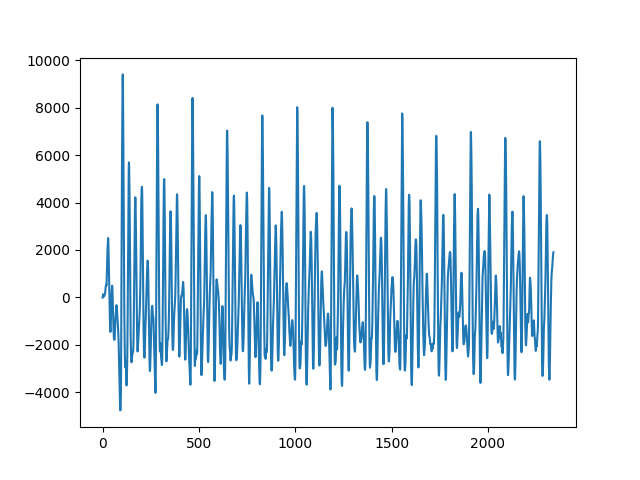
\includegraphics[height=6cm]{tser_sound_01.png}

Ses dalgalar� hakk�nda ilgin� bir g�zlem, e�er t�m ses dalgas�n� al�p yukar� ya
da a�a�� indirsem, seste hi�bir de�i�iklik olmuyor. 

\begin{minted}[fontsize=\footnotesize]{python}
wav1tmp = wav1 + 1000
plt.plot(wav1tmp)
fs = 16000 
scipy.io.wavfile.write('tmp10.wav', fs, np.array(wav1tmp))
\end{minted}

�stteki dosyadaki ses hala orijinali gibi. Ama e�er t�m ses verisini 100 ile
b�lseydim, bu ``ses k�smas�'' demek, ses duyulmayacakt�. 

\begin{minted}[fontsize=\footnotesize]{python}
tmp, wav2 = scipy.io.wavfile.read('phonemes/ah.wav')
plt.plot(wav2)
plt.savefig('tser_sound_02.png')
\end{minted}

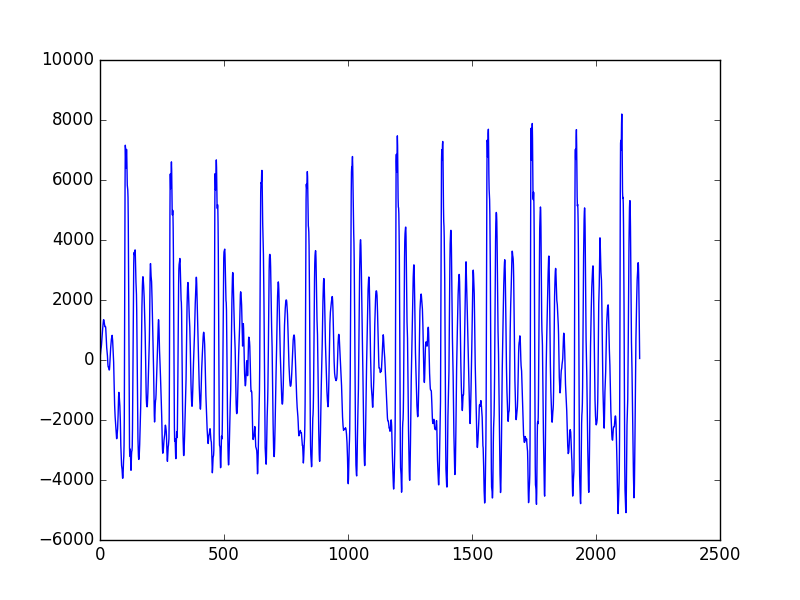
\includegraphics[height=6cm]{tser_sound_02.png}

Kendimiz sin�s bazl� ses yarat�yoruz,

\begin{minted}[fontsize=\footnotesize]{python}
import sounddevice as sd
T = 1.0    # seconds
t = np.linspace(0, T, int(T*fs), endpoint=False) 
x = np.sin(2*np.pi*440*t)
sd.play(x, fs)
scipy.io.wavfile.write('tmp.wav', fs, x)
tmp, wav3 = scipy.io.wavfile.read('tmp.wav')
plt.plot(wav3[:1000])
plt.savefig('tser_sound_03.png')
\end{minted}

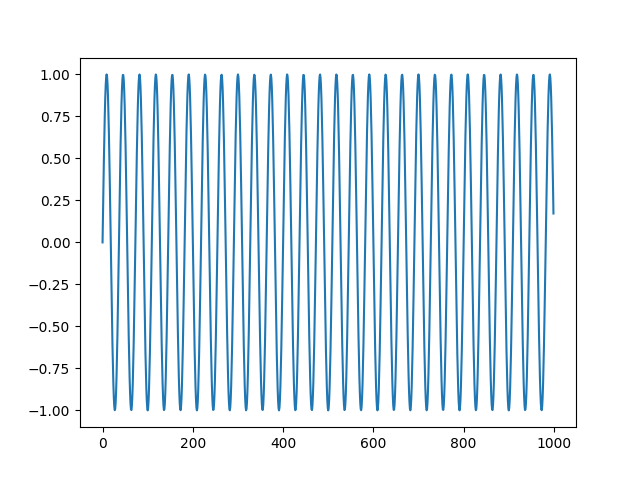
\includegraphics[height=6cm]{tser_sound_03.png}

�ki sin�s'� �st �ste koyal�m,

\begin{minted}[fontsize=\footnotesize]{python}
T = 1.0  
t = np.linspace(0, T, int(T*fs), endpoint=False) 
x = np.abs(np.sin(2*np.pi*440*t))
t = np.linspace(0, T, int(T*fs), endpoint=False) 
x2 = np.abs(np.sin(2*np.pi*220*t))
xx = x+x2
sd.play(xx, fs)
scipy.io.wavfile.write('tmp2.wav', fs, xx)
tmp, wav4 = scipy.io.wavfile.read('tmp2.wav')
plt.plot(wav4[:1000])
plt.savefig('tser_sound_04.png')
\end{minted}

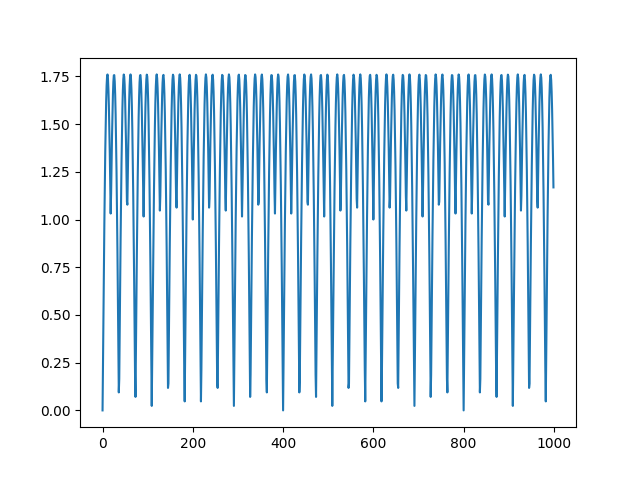
\includegraphics[height=6cm]{tser_sound_04.png}

Polis Sireni

\begin{minted}[fontsize=\footnotesize]{python}
y = sin(2*pi*1500*t - 100*sin(2*2*pi*t))
sd.play(y, fs)
\end{minted}


Fourier Analizi ile Sesi Sin�s E�rilerine Ay�rmak

\begin{minted}[fontsize=\footnotesize]{python}
fs = 16000
w = list(np.fft.fft(wav1))
freqs = np.fft.fftfreq(len(w))
max_freqs = []
for i in range(20):
     idx = np.argmax(np.abs(np.array(w)))
     freq = freqs[idx]
     del w[idx]
     freq_in_hertz = abs(freq * fs)
     max_freqs.append(freq_in_hertz)
print max_freqs
\end{minted}

\begin{verbatim}
[444.25459205467752, 451.08927808628789, 526.27082443400252, 546.77488252883393, 519.43613840239209, 553.60956856044425, 355.40367364374197, 403.24647586501493, 177.70183682187098, 239.21401110636481, 505.76676633917128, 580.94831268688597, 423.75053395984622, 512.60145237078166, 423.75053395984622, 526.27082443400252, 567.27894062366511, 683.46860316104232, 820.16232379325072, 950.0213583938488]
\end{verbatim}


\begin{minted}[fontsize=\footnotesize]{python}
T = 0.2
tmp = np.zeros((1,int(T*fs)))
for f in max_freqs: 
     t = np.linspace(0, T, int(T*fs), endpoint=False) 
     x = np.sin(2*np.pi*f*t)
     tmp += x
tmp = tmp * 500.
scipy.io.wavfile.write('tmp3.wav', fs, tmp[0])
import scipy.io.wavfile
tmp, wav11 = scipy.io.wavfile.read('tmp3.wav')
plt.plot(wav11)
plt.savefig('tser_sound_05.png')
\end{minted}

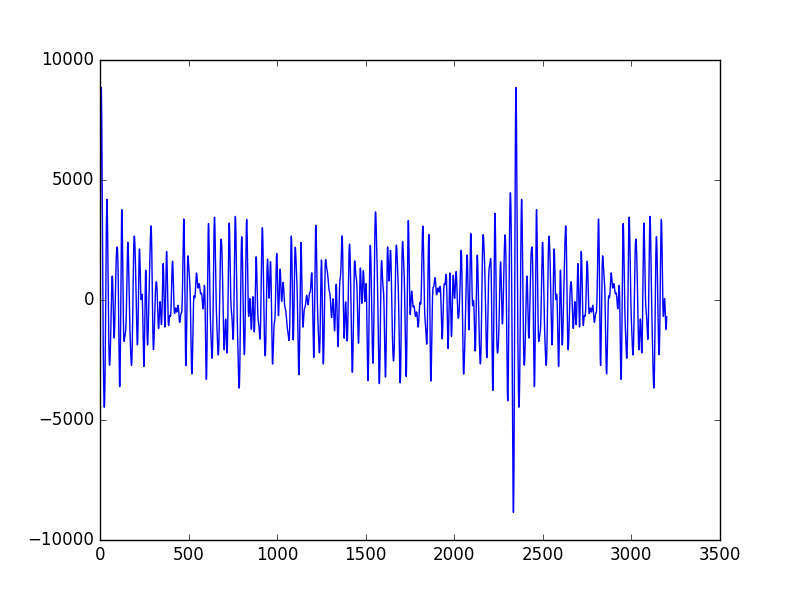
\includegraphics[height=6cm]{tser_sound_05.png}

Sinussel Regresyon ile Ayirmak

\begin{minted}[fontsize=\footnotesize]{python}
import statsmodels.api as sm
import pandas as pd

df = pd.DataFrame(wav1)
df.columns = ['wav']
tt = np.linspace(0,1,len(df))
for p in np.linspace(1,3,500):
   df['sin%f' % p] = np.sin(p*np.pi*df.index.astype(float))
   df['cos%f' % p] = np.cos(p*np.pi*df.index.astype(float))

X = sm.add_constant(np.array(df.drop(['wav'],axis=1)))
Y = df.wav.astype(float)
model = sm.OLS(Y,X)
results = model.fit()
print results.params[:5]
print results.pvalues[:5]
print 'R^2', results.rsquared
print len(df.columns[results.pvalues < 0.05])
print len(df)
\end{minted}

\begin{verbatim}
const   -1.840935e+00
x1      -3.832043e+13
x2       7.106000e+10
x3       8.083755e+13
x4      -9.566952e+12
dtype: float64
const    0.971236
x1       0.894484
x2       0.919536
x3       0.342939
x4       0.905573
dtype: float64
R^2 0.512162485291
48
2341
\end{verbatim}

E�er sesi olu�turmadan �nce �nemlili�i (significance) 0.05'ten b�y�k olan
katsay�lar� elersek, 

\begin{minted}[fontsize=\footnotesize]{python}
fs = 16000 
left = df.drop('wav',axis=1)
right = results.params
left = left.ix[:,df.columns[results.pvalues < 0.05]]
right = right[results.pvalues < 0.05]
print left.shape, right.shape
tmp = np.zeros((1,len(right)))
tmp[0,:] = right
dff = left.dot(tmp.T)
scipy.io.wavfile.write('tmp6.wav', fs, np.array(dff))
plt.plot(df.index,np.array(dff))
plt.savefig('tser_sound_06.png')
\end{minted}

\begin{verbatim}
(2341, 48) (48,)
\end{verbatim}

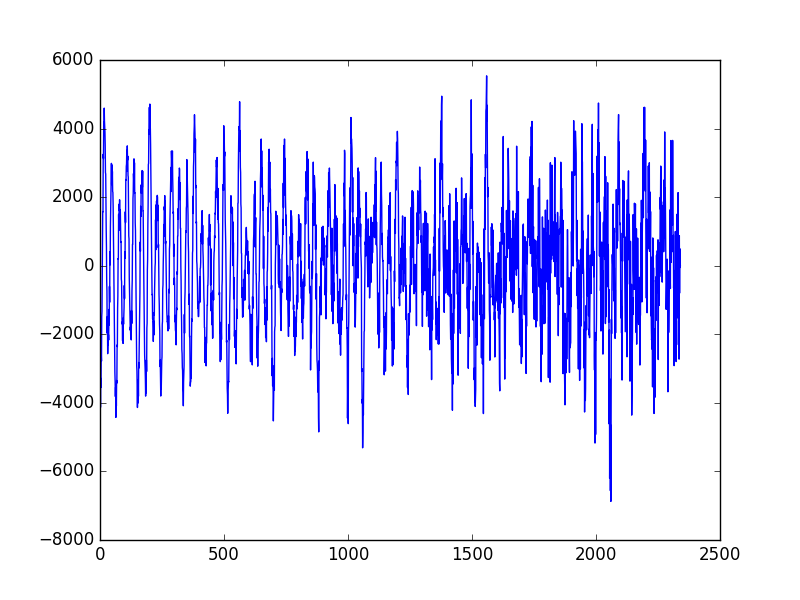
\includegraphics[height=6cm]{tser_sound_06.png}

Sesi dinleyince hafif bir benzerligin oldugunu duyuyoruz. 

Fonem Birlestirmek

Ufak bir deneme, fonemleri birlestirip kendi ismimi soyletmeye ugrastim.

\begin{minted}[fontsize=\footnotesize]{python}
import scipy.io.wavfile
tmp, wav5 = scipy.io.wavfile.read('phonemes/b.wav')
tmp, tmp2 = scipy.io.wavfile.read('phonemes/uh.wav')
wav5 = np.hstack((wav5,tmp2))
tmp, tmp2 = scipy.io.wavfile.read('phonemes/r.wav')
wav5 = np.hstack((wav5,tmp2))
tmp, tmp2 = scipy.io.wavfile.read('phonemes/r.wav')
wav5 = np.hstack((wav5,tmp2))
tmp, tmp2 = scipy.io.wavfile.read('phonemes/aa.wav')
wav5 = np.hstack((wav5,tmp2))
tmp, tmp2 = scipy.io.wavfile.read('phonemes/k.wav')
wav5 = np.hstack((wav5,tmp2))
tmp, tmp2 = scipy.io.wavfile.read('phonemes/k.wav')
wav5 = np.hstack((wav5,tmp2))
print len(wav5)
scipy.io.wavfile.write('tmp5.wav', 16000, wav5)
\end{minted}

\begin{verbatim}
14765
\end{verbatim}

Benim kendi sesimle kaydettigim 1. resimde gosterilen /ow/ sesi.

\begin{minted}[fontsize=\footnotesize]{python}
import scipy.io.wavfile
tmp, mywav = scipy.io.wavfile.read('my-ow.wav')
mywav = mywav[8000:12000]
plt.plot(mywav)
plt.savefig('tser_sound_07.png')
\end{minted}

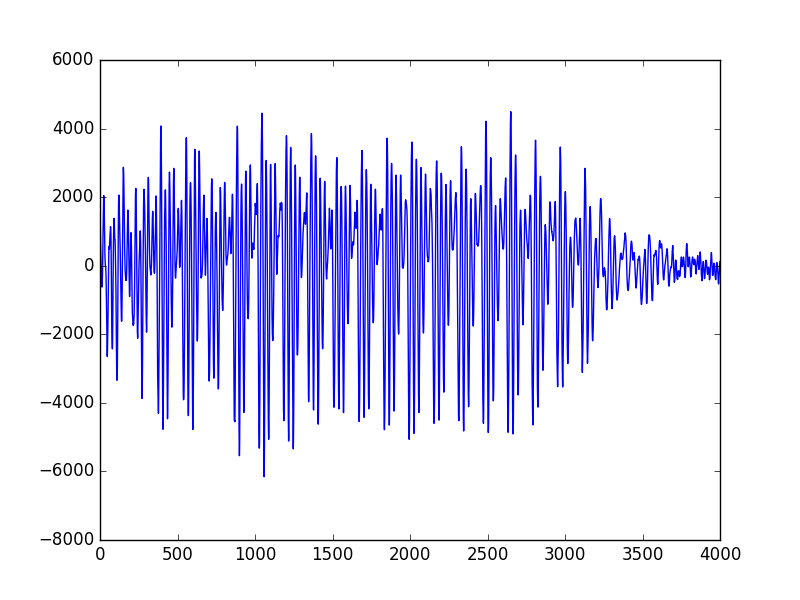
\includegraphics[height=6cm]{tser_sound_07.png}






\end{document}
